\documentclass[twocolumn]{article}
\usepackage{listings} %for listing code
\usepackage{multirow} %multirow cells in tables
\usepackage{geometry}	%
\usepackage{abstract} %to get email footnotes
\geometry{margin=2cm}	%more visible figures (more place) 
\usepackage[superscript,biblabel]{cite}%superscript citing
\usepackage[utf8]{inputenc}
\usepackage[english]{babel}
\usepackage{amsmath}	%booklet
\usepackage{hyperref}	%clickable citings, referencing URL via \url{}
\usepackage{siunitx}	%for SI units; see ftp://ftp.dante.de/tex-archive/macros/latex/exptl/siunitx/siunitx.pdf
\usepackage{graphicx} 	%includegraphics
\usepackage{mhchem}		%writing chemical elements with mass numbers
\usepackage[nottoc]{tocbibind}	%references
\usepackage{indentfirst}%indenting first paragraphs

%set code style

\lstset{		language=C++,
				frame=tb,
                basicstyle=\footnotesize\ttfamily,
                keywordstyle=\color{blue}\ttfamily,
                stringstyle=\color{red}\ttfamily,
                commentstyle=\color{green}\ttfamily,
                morecomment=[l][\color{magenta}]{\#},
                numbers=left
}


%the command \insertFigure{file} inserts figure with width 0.9*(column width)
\newcommand{\insertFigure}[1]{%
   \includegraphics[width=0.95\linewidth]{#1}%
}

\title{\textbf{E214: ATLAS}}
\author{Bence Mitlasóczki\thanks{s6bemitl@uni-bonn.de} and Beno\^it Scholtes\thanks{s6bescho@uni-bonn.de} \\ \textit{Rheinische-Friedrich-Wilhelms Universit\"at Bonn}}
\begin{document}
\renewcommand{\abstractname}{\vspace{-\baselineskip}} %supresses abstract title
\twocolumn[ %makes a one column abstract
\begin{@twocolumnfalse}
\maketitle
\begin{abstract} \vspace{-8mm}
Abstract goes here
\end{abstract}
\end{@twocolumnfalse}
\hspace{5mm} ]
\maketitle
\saythanks %from abstract package to ensure email footnotes from \thanks command in a two-collumn article
\section{Introduction}
Introduction text

The ATLAS detector is one of the several detectors in the LHC, a circular accelerator in Geneva, Switzerland. In it, two proton beams with the energy of 6.5~TeV each are collided with each other. The resulting legion %horde? multitude?
of particles are detected by the detectors. Out of these, the ATLAS (\textbf{A} \textbf{T}oroidal \textbf{L}HC \textbf{A}pparatu\textbf{S}) is the largest, general-purpose apparatus, able to detect the various particles created by the collisions. 

%TODO introduce acronyms: LHC
\section{Theory}
Our current best understanding of particle physics is the Standard Model of particle physics (SM). This model describes our discoveries of fundamental particles and their interactions with each other, mediated by fundamental forces. It furthermore describes the way these particles and forces combine to form atoms, from which many of the physical phenomena we encounter in everyday life can be explained. The main shortcoming of the SM however, is its inability to be united with gravity. That said, due to the relative weakness of gravity in comparison to the other fundamental forces, it rarely has an effect in particle physics and thus is mainly ignored (also in this paper).

\subsection{The Standard Model}
Figure~\ref{fig:part} give a summary of the particles in the SM with their most basic properties. Furthermore, there also exists anti-particles of many of these particles. An anti-particle, such as a positron, is identical to its particle (electron) apart from having the opposite electric charge. A neutral particle is often its own anti-particle such as the $Z^0$~boson, though neutrinos have anti-particles which are merely distinct by having opposing spin projections. All matter particles and the W~bosons have anti-particles while the rest are their own anti-particles.
\begin{figure}[!h]
	\centering
	\insertFigure{Images/SM.png}
	\caption{Illustration of the elementary particles in the SM. Quarks are in purple and Leptons in green, arranged into generation columns from left to right. The gauge bosons are in red, with the scalar Higgs boson in yellow.~\cite{part}}
	\label{fig:part}
\end{figure}
Quarks and leptons make up all the matter particles that have been discovered. These are given in three generations of particles, shown with the columns from left to right in the figure. Matter that is encountered everyday is largely structured from the first generation, namely the electron, electron neutrino, up quark, and down quark. For example, atoms are made up of electrons, protons, and neutrons, the latter two being composed of up and down quarks. The second and third generations are composed of particles which are otherwise exactly identical to their first generation counterpart apart from being heavier, the third generation being the heaviest of them all. This is only known to be true for the charged leptons (electron, muon, and tau) and quarks however. Though the neutrinos are known not to be massless, they have very small masses which have not been accurately measured. It is unknown which is the most massive and which the least.~\cite{Thompson} Figure~\ref{fig:mass} illustrates the relative masses of the matter particles.
\begin{figure}[!h]
	\centering
	\insertFigure{Images/mass.png}
	\caption{Illustration of the relative masses of the matter particles in their respective generations. The neutrinos are left blank to show that their masses are extremely small in comparison the other particles.~\cite{Thompson}}
	\label{fig:mass}
\end{figure}
The main reason why the second and third generation of particles are largely not existent in everyday phenomena is due to the requirement that higher energies are needed to produce these heavier particles. Furthermore, these heavier particles have shorter lifetimes due to their favourable decay into lighter particles, such as those in the first generation, due to the fundamental tendency of physical systems to higher kinetic energy states. Particle physics experiments need to be performed at increasingly higher energies in order to produce more massive particles that we do not readily observe. This is illustrated in Figure~\ref{fig:energy}. It should be noted that though neutrinos are not seen, trillions of solar neutrinos pass through your body each second, oscillating between their three different flavours.~\cite{Thompson} They are extremely difficult to detect due to the fact that they have a small mass and no electric charge. \\
\begin{figure}[!h]
	\centering
	\insertFigure{Images/energy.png}
	\caption{Illustration of the energies required to probe different structures and particles.~\cite{Thompson}}
	\label{fig:energy}
\end{figure}
\par Figure~\ref{fig:part} also shows the fundamental forces in the SM which are all mediated via the exchange of a gauge boson. The most familiar of these is the photon $\gamma$ which mediates the electromagnetic force. The photon interacts with all particles that have an electric charge and thus with all fundamental matter particles in the SM apart from the neutrinos. It also interacts with the W~bosons as they are electrically charged. The gluon gauge bosons mediate the strong force, thus called as it is the strongest force and binds nuclei and hadrons together, explained in Section~\ref{sec:hadrons}. The gluons interacts only with particles which have a so-called ``colour" charge, another property of particles similar to electric charge. Only quarks have a colour charge and the eight differently coloured gluons. Next, the oppositely charged W$^{\pm}$ and Z$^0$~bosons mediate the weak interaction, the weakest force apart from gravity. This force is responsible for radioactive decay and interacts with all matter particles in the SM. Finally, the Higgs boson is the most recently discovered particle which gives mass to all the matter particles in the SM by interacting with them.

\subsection{Hadrons and the Strong Force}\label{sec:hadrons}
Though quarks are elementary in the SM, they cannot be observed as free particles. This is because quantum chromodynamics (QCD) of the SM, the theory of the strong force, states that colour is confined such that systems with a colour charge cannot propagate freely, termed \textit{colour confinement}. Instead, only colourless composite particles can be observed. As a result, quarks form composite particles called hadrons which are bound by gluons. Hadrons generally form baryons, composed of three quarks, and mesons, composed of one quark and one anti-quark. The reason for the these two types is a result of there being three colours, red, blue, and green, for the quarks, and three anti-colours, anti-red, anti-blue, and anti-green, for the anti-quarks. Colourlessness is achieved by combining all three colours (or anti-colours) in a baryon, or a colour and its anti-colour in a meson, as shown in Figure~\ref{fig:colour}. Protons and neutrons are examples of baryons, composed of two up quarks and one down quark (written as uud), and two down quarks and one up quark (udd), respectively.
\begin{figure}[!h]
	\centering
	\insertFigure{Images/colour.png}
	\caption{Colour confinement resulting in baryons and mesons, given with some examples.~\cite{colour}}
	\label{fig:colour}
\end{figure}
Furthermore, exotic hadrons, which achieve colour confinement with more quarks, have been hypothesised and observed, though without explicit confirmation that the observations were indeed bound exotic hadrons~\cite{Thompson}. Examples include the tetraquark with two quarks and two respective anti-quarks, and the pentaquark with four quarks and an anti-quark. Exotic hadrons are rare however, due to the tendency of quarks to form and decay quickly into mesons and baryons.

\subsection{The Structure of Protons} 
The inner workings of hadrons need to be properly considered to accurately model hadronic interactions, expanding on the simplifications of the previous section. Importantly, there does not merely exist three \textsl{valence quarks} in baryons, those required to achieve colourlessness. Rather, the binding gluons also split into $q\overline{q}$ pairs, producing extra quarks called \textsl{sea quarks}~\cite{manual}. These gluons and sea quarks then carry part of the baryons momentum and it is these \textsl{partons} that interact with other particles. Figure~\ref{fig:parton} shows this phenomena in a proton-proton interaction.
\begin{figure}[!h]
	\centering
	\insertFigure{Images/parton.png}
	\caption{Feynman diagram of proton-proton collision, namely between a valence quark (top) and a sea quark. The two produced gluons here will immediately \textsl{hardonise}, form into hadrons, as a result of colour confinement. Thus, this interaction produces two protons and two hadron jets.~\cite{manual}}
	\label{fig:parton}
\end{figure}
In order to model collisions accurately, such as the proton-proton collisions at the LHC, the kinematics of the partons need to be used, derived from parton distribution functions (PDF). These functions describe relative momentum of the different partons as a fraction of the baryon's momentum. They are determined from experiments and depend on the energy scale of the interactions. At the energy scale of the LHC, most proton-proton interactions are of their sea quarks and not valence quarks~\cite{manual}. One needs to consider all possible reactions however and observe the products of the interaction, such as the number of jets and their momenta, to identify an interaction in a collider experiment.

\subsection{The Heavy Gauge Bosons}%Citation is for the numerical data
\subsubsection{Production, Detection}
The three massive gauge bosons in the Standard Model are the neutral Z$^0$ and the charged W$^\pm$ bosons. The Z$^0$ boson has a mass of $91.1876 \pm 0.0021$~GeV~\cite{manual}. The main decay mode is through jets ($\approx 70\%$). For our purposes, the decay to a lepton-antilepton pair (each lepton flavour having a branching ratio of $\approx 3.6-3.7 \%$) is the important mode, as it is easier to work with lepton tracks than jets. This is due to the large number of background QCD jets which are hard to distinguish from the Z$^0$ decay jets. The W$^\pm$ bosons have a slightly smaller mass of $80.403 \pm 0.029$~GeV. They decay to jets with the highest probability ($\approx 68 \%$), though the lepton-lepton ($e$, $\mu$) antineutrino decay modes are looked for in the experiment (the branching ratios are $\approx 10.6-11.3\%$ for each flavour) again due to their easy identification in the data. Both the W and Z bosons are produced in the weak Drell-Yan process, shown in Figure \ref{fig:WDiagram}.
\begin{figure} [!h]
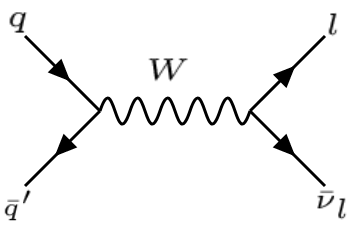
\includegraphics[scale=0.33]{Images/WDiagram.png}
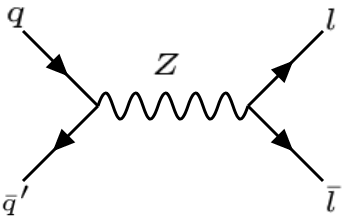
\includegraphics[scale=0.33]{Images/ZDiagram_differentflavour.png}
\caption{W and Z boson production and decay via the Drell-Yan process, from the interaction of a quark and anti-quark (not necessarily of the same flavour).}
\label{fig:WDiagram}
%Made with https://feynman.aivazis.com/
\end{figure}
The $Z^0 \rightarrow ee/\mu\mu$ processes can be precisely reconstructed from the ATLAS data, although there is a (suppressed) background from QED Drell-Yan pairs. In the case of $W \rightarrow e \bar{\nu}_e/\mu \bar{\nu}_\mu$ decays, the neutrino is not detected and its momentum needs to be reconstructed from the missing transverse momentum, as neutrinos are the mainly the only particle undetectable by the ATLAS detector. To a good approximation, both the Z and the W bosons decay at rest, thus the two final state particles have the same momentum, in the opposite direction. We will utilize the precisely known $Z^0$ mass for the verification of our method in Section~\ref{sec:Proc}, and consider the case of the W-boson mass below. 
\subsubsection{The Jacobi Peak}
%TODO not entirely clear why are we looking at d(sigma)/d(pT) and not sigma(pT), maybe because we are looking at bins, thus dsigma  ~ d(sigma)/d(pT)*d(pT)?
%TODO Check bibliography item WMassExperiment (correct form?)
In the process $W \, \rightarrow \, l \bar{\nu}_l$, the final state leptons have an approximate angular distribution~\cite{manual}
\begin{equation}
\frac{d\sigma}{d\cos \theta^*} = 1 + \cos^2 \theta^*, \nonumber
\end{equation}
where $\theta^*$ denotes the angle between the lepton track and the beam axis.
With this knowledge, we can calculate the differential cross-section
\begin{equation}
\frac{d \sigma}{d p_T} = \frac{d \sigma}{d \cos \theta^*} \left\vert \frac{d p_T}{d \cos \theta^*} \right\vert^{-1} = \frac{d \sigma}{d \cos \theta^*} \cdot  \frac{\frac{2p_T}{M_W}}{\sqrt{\left( \frac{M_W}{2}\right)^2 - p_T^2}}. \nonumber
\end{equation}
This curve clearly has a pole at $p_T = \frac{M_W}{2}$, called the Jacobi peak, and there should be no events with $p_T > \frac{M_W}{2}$ in a decay of the W-boson at rest. In reality, there are three distorting effects. Firstly, the detector is made of multiple parts each having a different sensitivity, or even not working, contributing to somewhat imprecise measured (and missing) momenta. Secondly, the W-boson mass has a Breit-Wigner type distribution centred at $M_W$ as it is not stable. The $p_T$ distribution should reflect this as well. Thirdly, the W-boson at the tree level has no transverse momentum (this assumption is made to derive the formula above), but the radiative corrections allow for some initial $p_T$. An example process is shown in Figure \ref{fig:WRadiation}. 
\begin{figure} [!h]
\centering
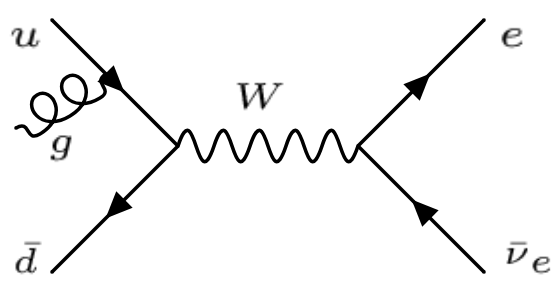
\includegraphics[scale=0.25]{Images/WRadiation.png}
\caption{Feynman diagram of a W-boson production with initial state radiation, giving the W-boson transverse momentum.}
\label{fig:WRadiation}
\end{figure}
\begin{figure} [!h]
\centering
\insertFigure{Images/WmassExample.eps}
\caption{An example of the expected electron transverse momentum histogram.\cite{WMassExperiment}}
\end{figure}
In the ideal case, one can easily declare the measured mass as the peak in the histogram. The distorting effects however smoothen out the curve complicating things. Instead, we take advantage of the available simulated data sets of decays of different particles with known masses. By fitting a function and extracting the transverse momentum corresponding to the half maximum, we can get a good estimation to what mass the half maximum of the real data fitting corresponds to. %TODO what kind of function do we fit? Give a bit more detail here about how we use this to obtain the mass of the W boson. Also, refer to Figure 8 if you use it.

\subsection{$Z^0$-Pair Production} %TODO I'm not sure about this section, it doesn't read well and doesn't really fit in to the report. Maybe put it after the next section or get rid of it. It doesn't go into enough detail to make it understandable.
Although we chose to determine the mass of the W-boson, here follows a short description of the other main task, searching for new physics phenomena in simulated data. The place to look in this case is the set of events where a $Z^0$ pair decays into four leptons, as this gives a clear signal of a ZZ event. The task here is to get rid of background events; these are a $t \bar{t}$ pair decaying via $t \rightarrow b W^+ \rightarrow b \, l^+ \nu_l$, or a Z boson with two additional b quarks (in both cases, B-hadrons that contain the b quarks might decay semi-leptonically, producing one more lepton each) with the help of data sets containing such events. After getting satisfactory filtering, a data set with SM and simulated Higgs or other "new physics" events; by looking at the characteristics of each hypothetical scenario (SUSY in the form of $Z Z^{(*)}$ events, new generation quarks, or additional gauge bosons ($Z^\prime$)), we need to decide which one might have appeared in the experiment.
\subsection{Extensions to the SM}
Though the SM has been extremely successful at describing fundamental physics, it has several shortcomings which necessitate explanations from new physics. Of these, some of the most significant are the inability of the SM to explain neutrino oscillations, gravity, dark matter, and the hierarchy problem. The latter is the observed discrepancy between the strengths of the fundamental forces. The strengths are quantified by coupling constants of the relevant gauge bosons with the relevant charge (gluons with colour charge) and these ``constants" actively depend on the energy scale of the interactions. That said, if a grand unified theory (GUT) of the three fundamental forces is to be established, whereby the forces are unified at some higher energy scale, it is expected that the strengths of the different coupling constants converge at this scale, a phenomena which is seemingly not achieved within the SM. \\
\par There are numerous theories which attempt to solve the different problems of the SM. One more promising theory is supersymmetry (SuSy) which proposes solutions to the hierarchy problem and provides a candidate dark matter particle. The minimal supersymmetric extension to the SM (MSSM) states that each lepton in the SM has a bosonic superpartner of spin 0, while every boson has a fermionic superpartner of spin 1/2. Figure~\ref{fig:susy} shows the MSSM particle spectrum.
\begin{figure}[!h]
	\centering
	\insertFigure{Images/susy.png}
	\caption{Particles in the MSSM.~\cite{susy}}
	\label{fig:susy}
\end{figure}
The superparticles have undefined mass, as MSSM particles of mass equal to their superpartners have not been found. As particle physics experiments such as the LHC have not found any MSSM particles yet, it is likely that they have much larger masses not probed yet by the LHC, if MSSM is indeed accurate. MSSM introduces a conserved and multiplicative quantum number called R-parity, defined as $R = (-1)^{3B+L+2S}$, where $B$ is baryon number, $L$ is lepton number, and $S$ is spin. SM particles have +1 R-parity while superparticles have -1 R-parity. As a result, a superparticle cannot decay into SM particles without violating R-parity. Thus, the lightest supersymmetric particle (LSP) must be stable. This is the natural dark matter particle candidate introduced by SuSy. Furthermore, with SuSy the three fundamental force coupling constants do indeed approximately unite at a scale of $10^{16}$~GeV, solving the hierarchy problem. Searching for evidence of SuSy is currently one of the main goals of the LHC as this would be a major leap in our understanding of physics. As of yet, no such signature have been observed. Other searches of new physics include additional heavy bosons proposed by other SM extension theories, such as bosons similar to the Z boson yet heavier. Furthermore, searches of higher generations of quarks and leptons in the SM are also conducted since they could very well exist yet are so massive that they have not been able to be produced in particle collisions. The LHC can easily investigate such proposals yet is limited in the energy of collisions and thus the masses of the produced particles.

\section{The ATLAS Detector}\label{sec:Exp}
This experiment analyses data from the ATLAS detector at the LHC. The ATLAS detector is cylindrical in shape, where the proton beams enter through each end of the cylindrical detector and collide in its centre. It makes use of numerous layers in order to detect particles produced in the collisions. Figure~\ref{fig:ATLAS} is a cross-sectional perspective of the detector showing the different layers. Circular detector disks are also added to the two ends of the cylindrical detector to further detect and measure particles at small angles to the beam axis.
\begin{figure}[!h]
	\centering
	\insertFigure{Images/ATLAS.png}
	\caption{Cross-sectional view of the ATLAS detector showing the different detectors at different layers and how different particles interact with the detectors. Most of the muon spectrometer is not included in this image.~\cite{manual}}
	\label{fig:ATLAS}
\end{figure}

\subsection{Inner Detector}
The inner detector helps determining the particle paths as precisely as possible. A solenoid magnet surrounds this system, creating a $\vec{B} = 2$~T magnetic field parallel to the colliding protons so as not to deflect them before collision. A particle with charge $q$ and velocity $\vec{v}$ in this magnetic field experiences a Lorentz force of 
\begin{equation}
\vec{F} = \frac{d}{dt} \vec{p} = q \vec{v} \times \vec{B}.\nonumber
\end{equation}
From the observed radius of the track of the particle, its momentum and charge sign can be determined allowing for a kinematic analysis of the collision. One can see in Figure~\ref{fig:ATLAS} how the charged particles are bent by the magnetic field in the inner detector. The inner detector is composed of different layers of detectors, hereby summarised:
\begin{itemize}
\item The innermost layer consists of over 80 million silicon semiconductor pixels (pixel detector, PD) which each have their own electronic circuit.~\cite{manual} This allows for precise spatial reconstruction of vertices, importantly being able to distinguish between closely separated primary and secondary vertices.
\item The semi-conductor tracker layer (SCT) serves the same purpose, but with long strips that make covering a larger surface area more practical.
\item The transition radiation tracker (TRT) consists of thin, long tubes (drift chambers) with inhomogeneous medium filling in the space between them. A particle passing through this medium emits transition radiation. The photons created this way, along with the particle itself, interact with the gas inside the tubes, causing ionizing. As there is a voltage applied to an electrode in the middle and the tube, the electrons are drawn to the electrode, contributing to an electric pulse. As the transition radiation is strongest for particles with high velocity, the strength of the signal can be used to identify the lightest particles, electrons and positrons.
\end{itemize}

\subsection{Outer Layers}
The layers surrounding the inner detector are largely used to determine the energies of the particles. It is composed of three sections.
\subsubsection{Electromagnetic Calorimeter}
The electromagnetic calorimeter (ECAL) is made of accordion-shaped lead and stainless steel sheets responsible for interacting electromagnetically with the particles passing through, creating an electromagnetic shower, seen in Figure~\ref{fig:ATLAS}. The liquid argon between the lead and steel sheets is ionized by the particles passing through, and the created free electrons are drawn to a copper electrode. An electromagnetic shower is caused by the radiation emitted from bremsstrahlung and compton scattering of the charged particle, whereby the emitted photons then pair-produce, which themselves emit radiation. This cycle continues until photons are emitted which aren't energetic enough to pair-produce. The shower of electron, positron, and photons produced are the electromagnetic shower, which deposits its energy in the detector allowing for a determination of the original particles energy. This calorimeter stops photons, electrons and positrons entirely and single handedly allows for a calculation of their energies. Hadrons and muons also deposit some energy here, but they pass through to reach the outer layers. The cooling system is a cryostat.

\subsubsection{Hadron Calorimeter}
The hadron calorimeter (HCAL) interacts strongly with the entering particles. The iron tiles induce hadronic showers, identical to the electromagnetic showers but caused hadrons colliding inelastically with the nuclei of the calorimeter material. The particles thus created enter the scintillation tiles producing light, and these photons are carried away in an optical fibre to a unit which measures light intensity, from which the deposited energy can be calculated. The scintillation material is liquid argon, so a cooling system is used in this layer as well. This calorimeter stops all hardons, leaving only muons and neutrinos to escape this layer of the detector.

\subsubsection{Muon Spectrometer}
The muon spectrometer is needed to measure the energy of the muons. The muons are so massive that they don't emit bremsstrahlung and don't interact strongly meaning that they only deposit a small amount of their energy in the previous layers of the detector. This unit is supplemented by a larger magnetic system consisting of toroidal magnets such that the detector is capable of determining the momentum of the muons independently of the inner layers. The tiles making up this layer consist of thin tubes filled with gas, and work on the principle of ionization, similarly to the TRT tubes. 

\section{Procedure} \label{sec:Proc}
\subsection{ATLANTIS}
As our first task, we looked at examples of events in the ATLAS detector in the event display software ATLANTIS. This way we got familiar with the working of the ATLAS detector and the signatures of different particles in the detector.
\begin{figure} [!h]
	\centering
	\insertFigure{Images/Atlantis_Electron_cropped.png}
	\caption{An (artificial) electron track as viewed in ATLANTIS, showing the electromagnetic shower in the ECAL (green).}
	\label{fig:elec}
\end{figure}

\subsubsection{Electron Energy}
We looked at the first 24 electron events in the learning data-set, determining the momentum by the track radius and the energy of the ECAL clusters by manually selecting the region. Figure~\ref{fig:elec} shows an example of an electron signature in ATLANTIS. The results are summed up in Table~\ref{tab:electron}. The histogram made of the energy/momentum ($E/p$) ratios is shown in Figure~\ref{fig:electron_histogram}. 24 events were chosen as four events were inconclusive as energy was not deposited, leaving 20 meaningful events.
\begin{figure} [!h]
\centering
\insertFigure{Images/electron_histogram.png}
\caption{Electron E/p histogram.}
\label{fig:electron_histogram}
\end{figure}

\begin{table} [!h]
\centering
\begin{tabular}{|c|c|c|c|}
\hline
\# & Momentum (GeV) & Energy (GeV) & E/p\\
\hline
1&	26.2&		54.7&	2.09\\\hline
2&	22.78&		35.2&	1.55\\\hline
3&	244.35&		223.2&	0.91\\\hline
4&	N/A &		N/A&	N/A\\\hline
5&	N/A	&		N/A&	N/A\\\hline
6&	66.67&		78.3&	1.17\\\hline
7&	7.55&		56.6&	7.50\\\hline
8&	129.82&		162.9&	1.25\\\hline
9&	3.27&		47.7&	14.59\\\hline
10&	79.01&		66.2&	0.84\\\hline
11&	95.93&		78.7&	0.82\\\hline
12&	37.4&		30.6&	0.82\\\hline
13&	89.35&		86.5&	0.97\\\hline
14&	235.24&		242.3&	1.03\\\hline
15&	105.14&		105.3&	1.00\\\hline
16&	N/A	  &		N/A&	N/A\\\hline
17&	28.62&		28.1&	0.982\\\hline
18&	53.41&		46.4&	0.869\\\hline
19&	32.92&		64.3&	1.95\\\hline
20&	105.64&		80.8&	0.765\\\hline
21&	N/A	  &		N/A&	N/A\\\hline
22&	93.52&		82.1&	0.878\\\hline
23&	113.98&		92.7&	0.813\\\hline
24&	155.35&		283&	1.82\\\hline
\end{tabular}
\caption{The momenta and energies of electrons, determined by the inner detector and ECAL, respectively. The E/p values are subsequently calculated.}
\label{tab:electron}
\end{table}
From the data, it can be seen that quite a few electrons were measured to have slightly higher momentum than energy, indicating the inaccuracy of the detector. The histogram shows that most electrons were measured with similar energy and momentum, though two relativistic electrons are found with E/p=7.50 and 14.59. A larger sample is required to determine the proper E/p distribution of electrons and whether a higher ratio of relativistic electrons are produced.

\subsubsection{Muon Momentum Comparison}
As our second task, we compared the measured muon momentum in the muon spectrometer and the inner detector. Calculating the differences between the two methods allowed us to determine the energy loss of the muons in the calorimeter and whether this depended on any quantity of the muons, such as their direction of flight. Table~\ref{tab:muon} provides the results. Figure~\ref{fig:muonat} shows a muon event in ATLANTIS.
\begin{table} [!h]
\centering
\begin{tabular}{|c|c|c|c|c|c|}
\hline
\multirow{2}{*}{\#} 	& I.D.		& M.C. 		& Diff. 	& \multirow{2}{*}{$\eta$} & \multirow{2}{*}{$\phi^{\circ}$}\\
					& (GeV)	& (GeV)	& (GeV)	&	&\\
\hline
1&	85.28&		53.92&		31.36&		1.437&	21\\\hline
2&	43.4&		43.83&		-0.43&		-0.767&	25\\\hline
3&	241.37&		237.02&		4.350&		-2.438&	230\\\hline
4&	48.89&		44.77&		4.12&		0.567&	311\\\hline
5&	168.16&		177.62&		-9.46&		-1.809&	244\\\hline
6&	117.32&		96.56&		20.76&		1.621&	152\\\hline
7&	71.94&		64.96&		6.98&		0.699&	3.8\\\hline
8&	199.91&		199.44&		0.470&		1.797&	67\\\hline
9&	57.84&		50.01&		7.830&		-0.287&	241\\\hline
10&	71.1&		0&			71.1&		1.181&	312\\\hline
11&	100.75&		94.11&		6.64&		-1.636&	48\\\hline
12&	38.26&		34.48&		3.78&		0.189&	326\\\hline
13&	105.19&		108.68&		-3.490&		1.163&	224\\\hline
14&	236.12&		263.61&		-27.49&		2.286&	103\\\hline
15&	131.69&		125.51&		6.180&		-1.763&	255\\\hline
16&	152.24&		157.69&		-5.450&		-1.874&	27\\\hline
17&	35.23&		32.18&		3.05&		0.395&	326\\\hline
18&	54.19&		50&			4.19&		0.229&	336\\\hline
19&	84.75&		68.09&		16.66&		0.773&	260\\\hline
20&	104.26&		107.98&		-3.72&		1.421&	78\\
\hline
\end{tabular}
\caption{The first column shows the Inner Detector measured momentum values, the second column the muon calorimeter momenta, the third column the loss of momentum (negative values show an increase in momentum), the fourth column $\eta$, the pseudorapidity, and the last column the azimuthal angle with respect to the proton beam axis.}
\label{tab:muon}
\end{table}
Here, we found that there are some cases where the muons seem to have gained momentum. This is indicative of the fact that the momenta of the muons are not accurately calculated in the inner detector due to the short pathlength of the muon in the detector and the insignificant deflection of the muon due to its large mass. As a result, the radius of the muon's arc cannot be precisely measured, thus resulting in an inaccurate measurement of the muons momentum. The muon system is much larger, on the other hand, allowing for a much more precise calculation of the muon momenta. Ultimately, the average energy loss of the muons in the calorimeter is 6.87~GeV. The possible dependence of the energy loss of the muons on their pseudorapidity $\eta$ and their azimuthal angles $\phi$ was analysed. These quantities were chosen as they were determined to be the only reasonable quantities that the measured energy loss could depend on. It was reasoned that the ends of the ATLAS detector, which are fitted with detector plates in which the calorimeters and muon system don't extend as far as in the middle cylindrical section, won't be able to measure the muon momenta as accurately, or that the muons won't dispose as much energy in the shortened calorimeter. That said, no dependence on these quantities was found in the energy loss of the muons. This could either be because there is no such correlation to be found or that a large sample size is required. A larger sample size could be needed as the accuracy of the measured muon momenta is not very high, resulting in fluctuations in the energy differences calculated which obscure any $\eta$ or $\phi$ dependence. A large sample size could counteract this obscurity.
\begin{figure} [!h]]
\centering
\insertFigure{Images/Atlantis_Muon_cropped.png}
\caption{Artificial muon event as seen in ATLANTIS (the panel with quantitive informations has been cropped for better visibility).}
\label{fig:muonat}
\end{figure}

\subsection{Electron energy calibration}
As the detector is not ideal, we need to calibrate the different regions to account for the differences in their characteristics. We chose sections of $\Delta \eta = 1.25$ and $\Delta \varphi = \pi/2$ ($-2.5 \leq \eta \leq 2.5$, $-\pi < \varphi < \pi$). Using the well-known Z$^0$ mass, we used cuts to limit ourselves to each of these intervals and iterated the process of scaling the individual values. We also introduced a transverse momentum dependent correction, finally a constant shift. Our final \textsl{ElecCalib.C} contents can be seen in Section \ref{sec:Code}. The mass obtained after three iterations is $91.1975 \pm 0.0204$~GeV, with resolution $2.5315 \pm 0.0251$, we considered this precise enough for our purposes. Figure \ref{fig:final_iteration} shows our fitting.
\begin{figure}
\centering
\insertFigure{Images/FinalIteration.png}
\caption{Final iteration fitting of Z$^0$}
\label{fig:final_iteration}
\end{figure}
\subsection{Measurement of the W-boson mass}
\begin{figure}
\centering
\insertFigure{Images/FirstWFit.png}
\caption{Z$^0$ mass from ATLAS data}
\label{fig:Z0ATLAS}
\end{figure}
After setting up the electron energy calibration file, we tested it on real ATLAS data, as seen in Figure \ref{fig:Z0ATLAS}. The mass acquired here is in good agreement with the commonly accepted value. As our next step, we tried scaling the QCD background by comparing the ATLAS data points and our stack-plot. We decided that the scale factor $\alpha = 0.35 \pm 0.05$ gave a fair match (the error was approximated by manual trial).
\begin{figure}
\centering
\insertFigure{Images/ptw_scale.png}
\caption{QCD scaled to achieve (by eye) a good match between the stack-plot and the data points.}
\label{fig:QCDscalefactor}
\end{figure}
Following the guide, we then set up a macro file to visualize the effect of our cuts on the different data sets of W-boson events with different masses, all at once. The measured half maxima and a linear fitting is shown in Figure \ref{fig:gaugecurve}. We found the linear fitting to be
\begin{equation}\nonumber
\text{HM}(m) = (0.50267 \pm 0.00867)\cdot m + (2.2613 \pm 0.6898)
\end{equation}
For the real data, we obtained the half max to be at $43.04 \pm 0.09$, which gives, after inverting the previous relation, a mass of $m_\text{W} = 81.12 \pm 2.03$~GeV.
%TODO maybe use inverted data as original fitting? Then need to figure out how to fit when x-axis has errors.
\begin{figure}
\centering
\insertFigure{Images/Jacobihalfmax.png}
\caption{The gauge curve data points with linear fitting.}
\label{fig:gaugecurve}
\end{figure}
\subsection{Cross-check using ATLAS \textit{ee} pair data}
The gauge curve can be applied in the case of data for electron-positron pairs. 
\begin{figure}
\centering
\insertFigure{Images/ZeeCheck.png}
\caption{Plot showing the cross-check procedure.}
\label{fig:crosscheck}
\end{figure}
Using the inverse of the gauge function again, we get
\begin{equation}
HM^{-1} \big(48.47 \pm 0.12\big) = 91.927 \pm 2.171 \, \text{GeV,}
\end{equation}
in good agreement with the literature value, which supports our previous works.
\subsubsection{Error sources}
\section{Conclusion}
\begin{thebibliography}{9}
\bibitem{Thompson}
M. Thompson, \textsl{Modern Particle Physics} (Cambridge University Press, New York, 2013).
\bibitem{part}
T. DeMichele, \textit{The Standard Model (of Particle Physics) Explained}, WWW Document, \url{http://factmyth.com/the-standard-model-of-particle-physics-explained/}.
\bibitem{colour}
H. Klus, \textit{The Strong Nuclear Force}, WWW Document, \url{http://www.thestargarden.co.uk/Strong-nuclear-force.html}.
\bibitem{pseudo}
J. Denker, \textit{Quarks -\textgreater Mesons -\textgreater Nonet = Octet plus Singlet}, WWW Document, \url{https://www.av8n.com/physics/quark-meson-nonet.htm}.
\bibitem{manual}
Unspecified author, \textsl{Advanced Laboratory Course physics601:E214 The ATLAS Experiment} (University of Bonn, 2018).
\bibitem{WMassExperiment}
%Chris Hays, Ashutosh Kotwal, Larry Nodulman, Oliver Stelzer-Chilton, William Trischuk, Ian Vollrath, https://www-cdf.fnal.gov/physics/ewk/2007/wmass/
Hays, C., Kotwal, A., Nodulman, L., Stelzer-Chilton, O., Trischuk, W., Vollrath, I. (2007). \textsl{First Measurement of the W Boson Mass with CDF in Run II}.
\bibitem{susy}
Unspecified author, \textsl{Extensions to the Standard Model?}, WWW Document, \url{http://www.physics.gla.ac.uk/ppt/bsm.htm}.
\bibitem{booklet}
Unspecified author, \textsl{Advanced Laboratory Course (physics601): Description of Experiments} (University of Bonn, 2018).
\bibitem{youtube}
ATLAS Experiment YouTube channel, \url{http://youtube.com/TheATLASExperiment}.
 \bibitem{link}
 W. U. Boeglin, \textit{Scintillation Detectors}, WWW Document, \url{http://wanda.fiu.edu/teaching/courses/Modern_lab_manual/scintillator.html}.
\bibitem{pdf_on_website}
Unspecified author, \textsl{Gamma Ray Spectroscopy} (University of Florida, 2013), \url{https://www.phys.ufl.edu/courses/phy4803L/group_I/gamma_spec/gamspec.pdf}.
\bibitem{cfd}
E. Ermis and C. Celiktas, International Journal Of Instrumentation Science 1, (2013), pp.54-62.
%alternative url: https://en.wikipedia.org/wiki/Constant_fraction_discriminator
\bibitem{leo}
W. R. Leo, \textsl{Techniques for Nuclear and Particle Physics Experiments} (Springer-Verlag, 1987), p. 305.
%William R. Leo
\bibitem{meliss}
A. C. Melissinos, J. Napolitano, \textsl{Experiments in Modern Physics, 2\textsuperscript{nd} edition} (Academic Press, San Diego, 2003), pp 419-21.
\end{thebibliography}
\newpage
\onecolumn
\section{Code}\label{sec:Code}
%TODO this does not look too nice -- It's fine! :P
\begin{lstlisting}
#include "math.h"
#include "TMath.h"

double ElecCalib(double e_raw, double pt, double eta, 
		 double phi, double etiso, double eoverp, double mindrjet)
{
  //double dummy=pt*eta*phi*etiso*eoverp*mindrjet;
  double energy = e_raw ;
    
if (eta>-2.5 && eta<-2.5/2){
    if (phi> -3.14 && phi< -3.14/2) energy = energy *(91.2/89.79)*(91.19/91.19)*(91.19/91.17);
    else if (phi> -3.14/2 && phi< 0) energy = energy *(91.2/89.76)*(91.19/91.23)*(91.19/91.18);
    else if (phi> 0 && phi< 3.14/2) energy = energy *(91.2/89.69)*(91.19/91.14)*(91.19/91.18);
    else if (phi> 3.14/2 && phi< 3.14) energy = energy *(91.2/89.6)*(91.19/91.09)*(91.19/91.13);
}
else if (eta>-2.5/2 && eta<0){
    if (phi> -3.14 && phi< -3.14/2) energy = energy *(91.2/89.84)*(91.19/91.17)*(91.19/91.15);
    else if (phi> -3.14/2 && phi< 0) energy = energy *(91.2/89.72)*(91.19/91.13)*(91.19/91.17);
    else if (phi> 0 && phi< 3.14/2) energy = energy *(91.2/90.11)*(91.19/91.3)*(91.19/91.25);
    else if (phi> 3.14/2 && phi< 3.14) energy = energy *(91.2/89.92)*(91.19/91.22)*(91.19/91.22);
}
else if (eta>0 && eta<2.5/2){
    if (phi> -3.14 && phi< -3.14/2) energy = energy *(91.2/89.86)*(91.19/91.13)*(91.19/91.16);
    else if (phi> -3.14/2 && phi< 0) energy = energy *(91.2/89.96)*(91.19/91.22)*(91.19/91.22);
    else if (phi> 0 && phi< 3.14/2) energy = energy *(91.2/89.73)*(91.19/91.12)*(91.19/91.16);
    else if (phi> 3.14/2 && phi< 3.14) energy = energy *(91.2/89.91)*(91.19/91.16)*(91.19/91.20);
}
else if (eta>2.5/2 && eta<2.5){
    if (phi> -3.14 && phi< -3.14/2) energy = energy *(91.2/89.92)*(91.19/91.23)*(91.19/91.22);
    else if (phi> -3.14/2 && phi< 0) energy = energy *(91.2/90.01)*(91.19/91.16)*(91.19/91.23);
    else if (phi> 0 && phi< 3.14/2) energy = energy *(91.2/89.82)*(91.19/91.16)*(91.19/91.18);
    else if (phi> 3.14/2 && phi< 3.14) energy = energy *(91.2/89.91)*(91.19/91.12)*(91.19/91.21);
}

if (fabs(pt)>0 && fabs(pt)<20) energy = energy*(91.19/89.26)*(91.19/90.04);
else if (fabs(pt)>20 && fabs(pt)<30) energy = energy*(91.19/90.13)*(91.19/90.79);
else if (fabs(pt)>30 && fabs(pt)<35) energy = energy*(91.19/90.51)*(91.19/90.92);
else if (fabs(pt)>35 && fabs(pt)<40) energy = energy*(91.19/90.68)*(91.19/90.86);
else if (fabs(pt)>40 && fabs(pt)<45) energy = energy*(91.19/91.32)*(91.19/91.1);
else if (fabs(pt)>45 && fabs(pt)<50) energy = energy*(91.19/92.34)*(91.19/91.75);
else if (fabs(pt)>50 && fabs(pt)<60) energy = energy*(91.19/92.31)*(91.19/91.92);
else if (fabs(pt)>60) energy = energy*(91.19/91.89)*(91.19/91.85);

energy = energy - 0.025;


  // if (fabs(eta)>1.5) energy = energy * 91.2/78.2;
  // else if (fabs(eta)>2.0) energy = energy * 91.2/85.4;
return energy;
} 
\end{lstlisting}
\newpage
\end{document}